


%\bf{摘要:} 本文提出一种

%\noindent 中文字体(默认宋体)\\
%\fangsong 中文字体(仿宋) \songti 中文字体(宋体) \lishu 中文字体(隶书) \heiti 中文字体(黑体)\\
%\CJKfamily{zhkai} 中文字体(楷书) \CJKfamily{zhyou} 中文字体(幼圆) \CJKfamily{zhyahei} 中文字体(微软雅黑)\\


\textbf{Abstract: }Abstract Abstract Abstract Abstract Abstract Abstract Abstract .

\textbf{Keywords: }Keywords, Keywords, Keywords, Keywords.

% \textbf{Abstract:} AbstractAbstractAbstractAbstractAbstractAbstractAbstractAbstractAbstractAbstractAbstractAbstractAbstractAbstractAbstract.

% \textbf{keywords: }keywords, keywords, keywords, keywords.
\setlength{\parindent}{2em} 
\section{Introduction}
\label{intro}
The ducted fan unmanned aerial vehicle (UAV) is the aircraft that the propeller/rotor/fan is installed inside a circular duct while control vanes are involved to stabilize the attitude of the vehicle, as show in Fig.\ref{fig:1}. 
	
	In the earlier works on the ducted fan UAV control\cite{RN35,RN45}. 
	
	\begin{figure}[tb]
		\centering
		\includegraphics[width=3.2in]{Fig/Fig1.eps}
		\caption{Ducted fan UAV, weighing $1.5 kg$ and configured with a $9 inch$ ducted rotor, which equipped with {\it PX4} autopilot. Details about the experiments are shown in this video\protect\footnotemark[1].}
		\label{fig:1}     
	\end{figure}
	\footnotetext[1]{\url{https://youtu.be/978SQ7nIA50}}
	
	This paper proposes a prioritized control allocation algorithm in which the control allocation problem is solved by an optimization technique. 	
	
	The contributions of this work are:
	\begin{enumerate}
		\item An angular velocity.
		
		\item A algorithm is proposed to solve.
		
		\item Combine. We release our implementation as open-source software\footnote[2]{Source code of the proposed method will be released in \url{https://github.com} after the publishing of this paper.}, which includes a simulation that enables more experimentation.
	\end{enumerate}

\section{Ducted Fan Modeling}
Modeling
\section{Results}
\subsection{Experiment 1} 
	\label{Experiment_1}
	The results of experiment 1 are presented in Fig.\ref{fig:6}, in which Fig.\ref{fig:6} \subref{fig:6:a} \subref{fig:6:b} \subref{fig:6:c} are the results in the absence of  the actively produced disturbance, while Fig.\ref{fig:6} \subref{fig:6:d} \subref{fig:6:e} \subref{fig:6:f} are the results under the actively produced disturbance. Obviously, we can state that the overall control performance is less satisfactory under the PID controller. 
	
	Furthermore, contrast to the PID controller, it seems that the introduction of the disturbance affects nothing on the system responses under the INDI controller. With and without the disturbance, the tracking performance shows no difference on each attitude channel. This is due to the fact that INDI is capable of estimating and compensating the exogenous disturbance instantly, while PID acts mush slower since it relies on the accumulation of the tracking error. In all, it is revealed that the proposed INDI controller can achieve well tracking performance with excellent disturbance rejection ability.
	\begin{figure*}
		\centering
		\subfloat[Roll channel without disturbance]{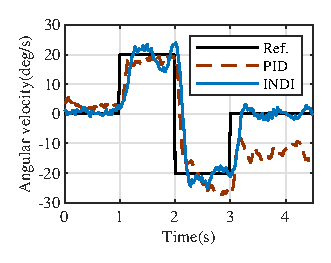
\includegraphics[scale=1]{Fig/Fig6a.eps}%
			\label{fig:6:a}}\hfil   %or  \quad
		\subfloat[Pitch channel without disturbance]{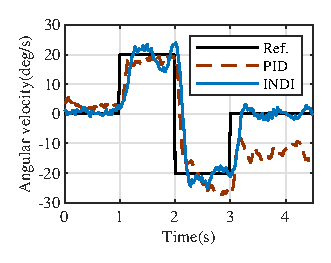
\includegraphics[scale=1]{Fig/Fig6a.eps}%
			\label{fig:6:b}}\hfil
		\subfloat[Yaw channel without disturbance]{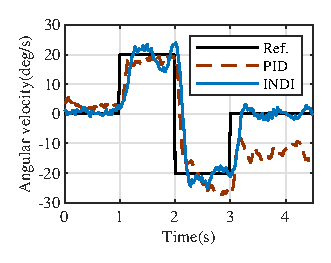
\includegraphics[scale=1]{Fig/Fig6a.eps}%
			\label{fig:6:c}}\\
		\subfloat[Roll channel with disturbance]{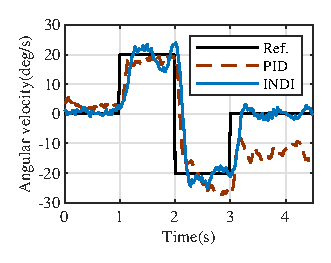
\includegraphics[scale=1]{Fig/Fig6a.eps}%
			\label{fig:6:d}}\hfil
		\subfloat[Pitch channel with disturbance]{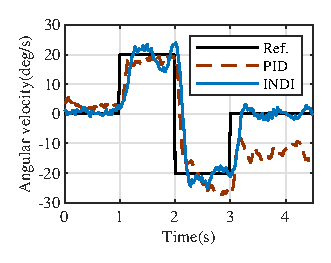
\includegraphics[scale=1]{Fig/Fig6a.eps}%
			\label{fig:6:e}}\hfil
		\subfloat[Yaw channel with disturbance]{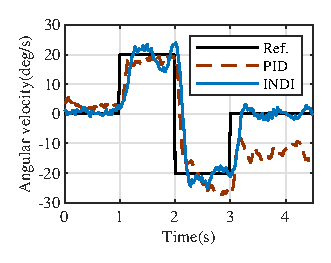
\includegraphics[scale=1]{Fig/Fig6a.eps}%
			\label{fig:6:f}}
		\caption{\label{fig:6}Results of experiment 1}
	\end{figure*} 
	Furthermore, 
\newpage

